\documentclass[aspectratio=169]{beamer}
\usetheme{Madrid}
\usecolortheme{default}

\usepackage{fontspec}
\usepackage{polyglossia}
\setmainlanguage{english}
\usepackage{graphicx}
\usepackage{amsmath}
\usepackage{booktabs}
\usepackage{xcolor}

\definecolor{examplecolor}{RGB}{180,83,9}

\setbeamertemplate{navigation symbols}{}
\setbeamertemplate{footline}[frame number]
\setbeamerfont{footnote}{size=\tiny}

\newcommand{\fuente}[1]{{\footnotesize\textit{Source: #1}}}
\newcommand{\ejemplo}[1]{\par\vspace{0.4em}{\small\color{examplecolor}\textbf{Example:} #1}}

\title[2. Supervised Learning]{Chapter 2: Supervised\\Learning}
\subtitle{Course material}
\author{Universidad de Salamanca}
\institute{Faculties of Sciences and Chemical Sciences}
\date{\today}

\begin{document}

% ============================================================
\begin{frame}
  \titlepage
\end{frame}

\begin{frame}{In this chapter}
  \begin{enumerate}
    \item \textbf{2.1 Regression}: predicting a continuous value
    \begin{itemize}
      \item Linear regression, least squares, gradient descent
      \item Regularization: Ridge, Lasso, Elastic Net
    \end{itemize}
    \item \textbf{2.2 Classification}: predicting a category
    \begin{itemize}
      \item Logistic regression, trees, Random Forest, SVM
      \item Ensembles, neural networks, and how to evaluate them
    \end{itemize}
  \end{enumerate}
\end{frame}

\begin{frame}{What is supervised learning?}
  \begin{itemize}
    \item We have \textbf{data} (input features, $X$) and \textbf{labels} (correct answers, $y$)
    \item The goal is to learn the relationship $X \rightarrow y$
    \item It's like learning with a ``supervisor'' who corrects your answers during training
  \end{itemize}
  \vspace{1em}
  \begin{columns}
    \begin{column}{0.5\textwidth}
      \textbf{Regression} (continuous value)
      \begin{itemize}
        \small
        \item House price
        \item Tomorrow's temperature
      \end{itemize}
    \end{column}
    \begin{column}{0.5\textwidth}
      \textbf{Classification} (category)
      \begin{itemize}
        \small
        \item Is this email spam?
        \item Is this image a cat, dog, or bird?
      \end{itemize}
    \end{column}
  \end{columns}
\end{frame}

% ============================================================
\section{2.1 Regression}

\begin{frame}{Linear regression}
  \begin{itemize}
    \item \textbf{Simple}: a single predictor, $Y \approx \beta_0 + \beta_1 X$
    \item \textbf{Multiple}: one coefficient per feature, $Y = \beta_0 + \beta_1X_1 + \dots + \beta_pX_p + \epsilon$
    \item $\beta_0$ (intercept) and $\beta_1 \dots \beta_p$ (weights) are what the model learns from the data
    \item In $p$ dimensions, the model represents a \textbf{hyperplane}
  \end{itemize}
  \begin{center}
    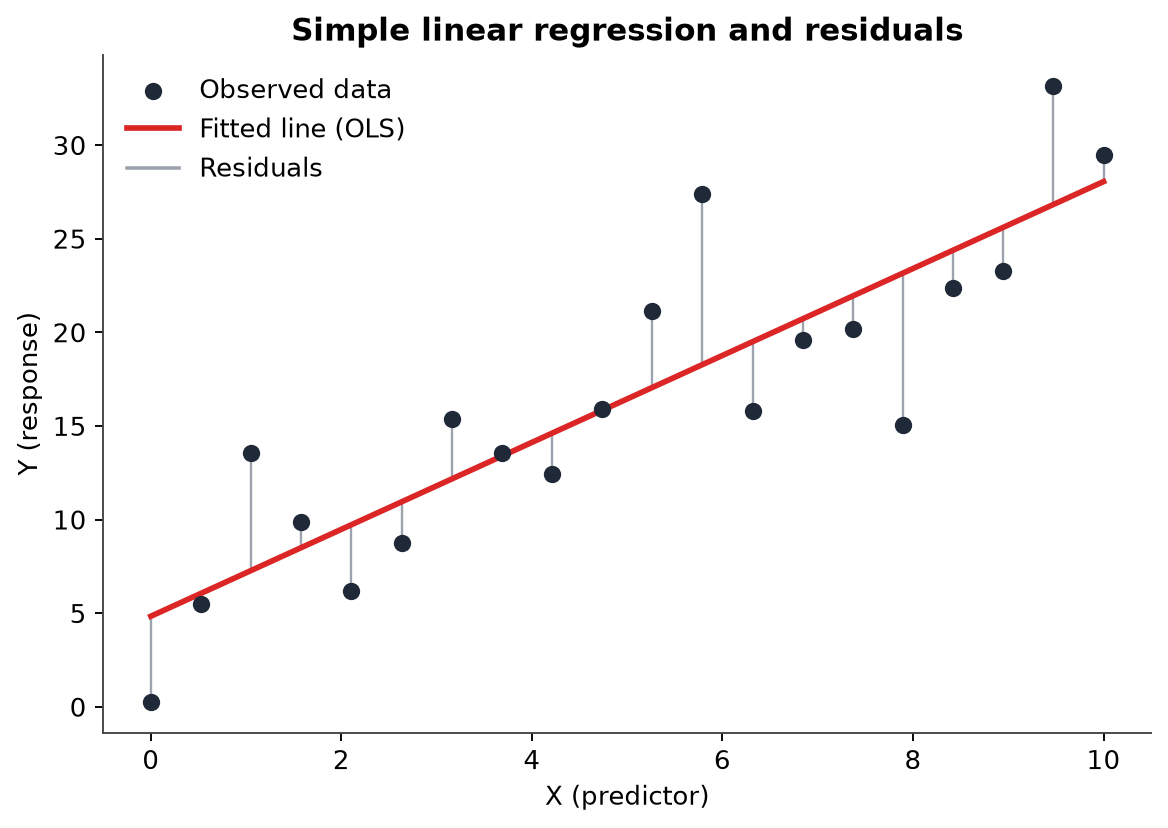
\includegraphics[width=0.5\textwidth]{../book/_static/generated/figures/en/linear_regression_fit.png}
  \end{center}
\end{frame}

\begin{frame}{Real example: the \textit{Advertising} dataset}
  \begin{itemize}
    \item Predicts \textit{Sales} from TV, radio, and newspaper advertising spend
    \item The line minimizes the sum of squared residuals (OLS)
  \end{itemize}
  \begin{center}
    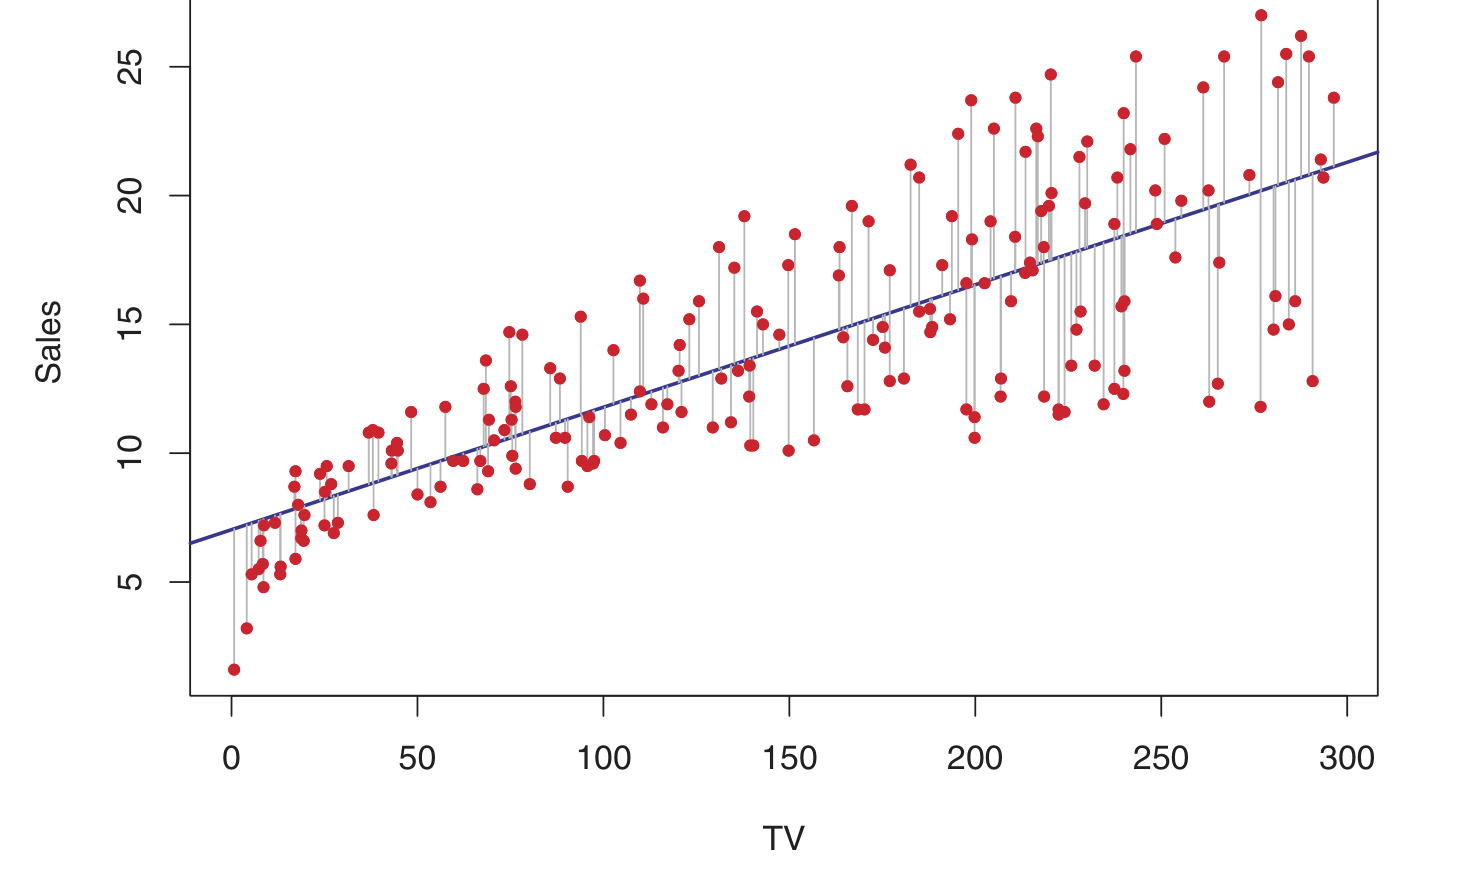
\includegraphics[width=0.48\textwidth]{../book/_static/book_figures/islr_fig3_1_advertising.png}
  \end{center}
  \fuente{James, Witten, Hastie \& Tibshirani (2013), \textit{An Introduction to Statistical Learning}, Fig. 3.1. Freely distributed textbook (statlearning.com).}
\end{frame}

\begin{frame}{Ordinary Least Squares (OLS)}
  \begin{itemize}
    \item A \textbf{residual} $e_i = y_i - \hat{y}_i$ is the difference between the real and predicted value
    \item OLS finds the weights that \textbf{minimize} the sum of squared residuals: $RSS = \sum_{i=1}^{n}(y_i-\hat{y}_i)^2$
    \item It has an \textbf{exact analytical solution}: $\hat{\beta} = (X^TX)^{-1}X^Ty$
    \item Geometric view: $\hat{y}$ is the orthogonal projection of $y$ onto the space spanned by $X$
  \end{itemize}
  \ejemplo{with just 3 houses (m\textsuperscript{2} and price), OLS finds in a single step the line that best summarizes that relationship --- no trial and error needed.}
\end{frame}

\begin{frame}{Gradient descent}
  \begin{itemize}
    \item When data is massive, solving the exact equation is too costly
    \item \textbf{Iterative} algorithm: starts from random weights and nudges them toward lower error, step by step
    \item $\theta \leftarrow \theta - \alpha \nabla J(\theta)$, where $\alpha$ is the \textbf{learning rate}
    \item Variants: \textit{Batch} (whole dataset), \textit{Stochastic} (one sample), \textit{Mini-batch} (a small group)
  \end{itemize}
  \ejemplo{\footnotesize it's like walking down a foggy mountain: at each step you feel the slope under your feet and move toward where it descends most, until you reach the valley.}
  \begin{center}
    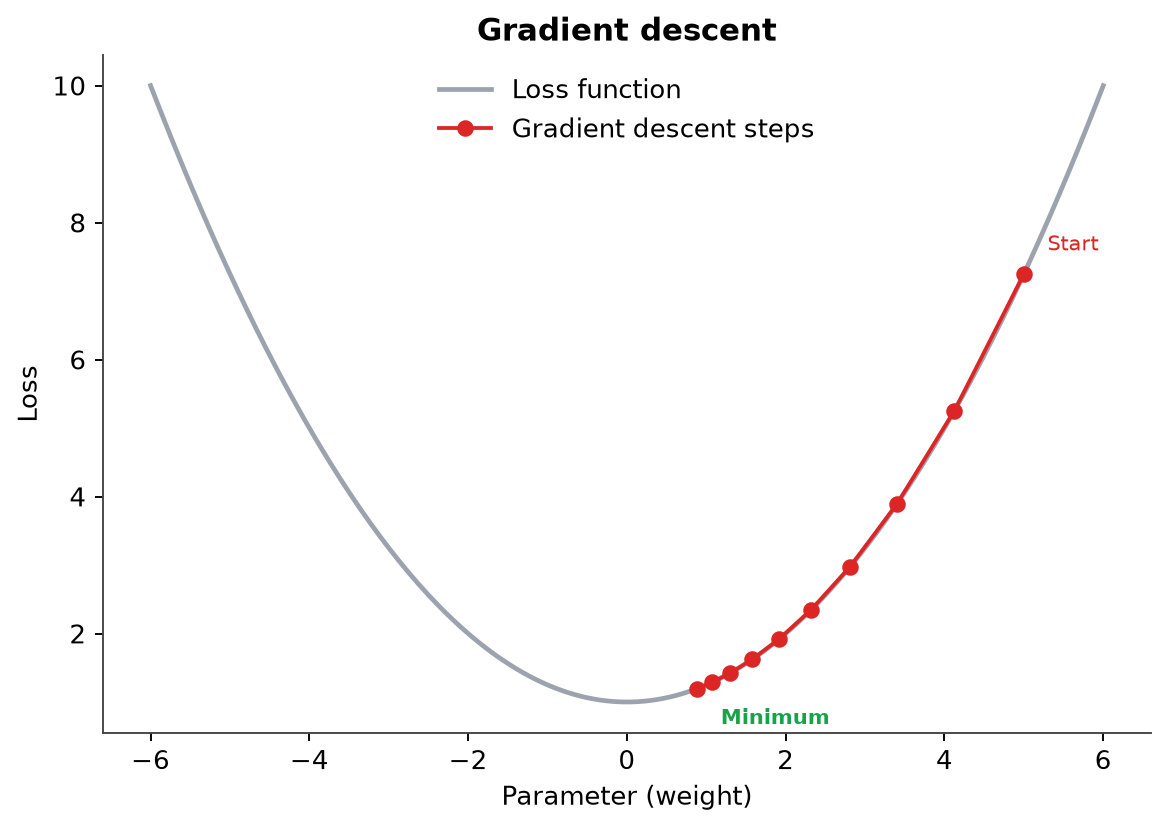
\includegraphics[width=0.32\textwidth]{../book/_static/generated/figures/en/gradient_descent.png}
  \end{center}
\end{frame}

\begin{frame}{Polynomial regression and the risk of overfitting}
  \begin{itemize}
    \item Powers of the original predictors ($X^2$, $X^3$...) are added to capture curves
    \item Still a model that is \textbf{linear in its parameters} --- can still be trained with OLS
    \item The higher the degree, the higher the risk of memorizing noise (overfitting)
  \end{itemize}
\end{frame}

\begin{frame}{Regularization: Ridge and Lasso}
  \begin{itemize}
    \item Penalize large weights in the cost function, forcing simpler models
    \item \textbf{Ridge} ($L_2$): penalizes $\sum \beta_j^2$ --- shrinks coefficients without zeroing them
    \item \textbf{Lasso} ($L_1$): penalizes $\sum |\beta_j|$ --- can push coefficients exactly to zero (variable selection)
    \item \textbf{Elastic Net}: combines both penalties
  \end{itemize}
  \begin{center}
    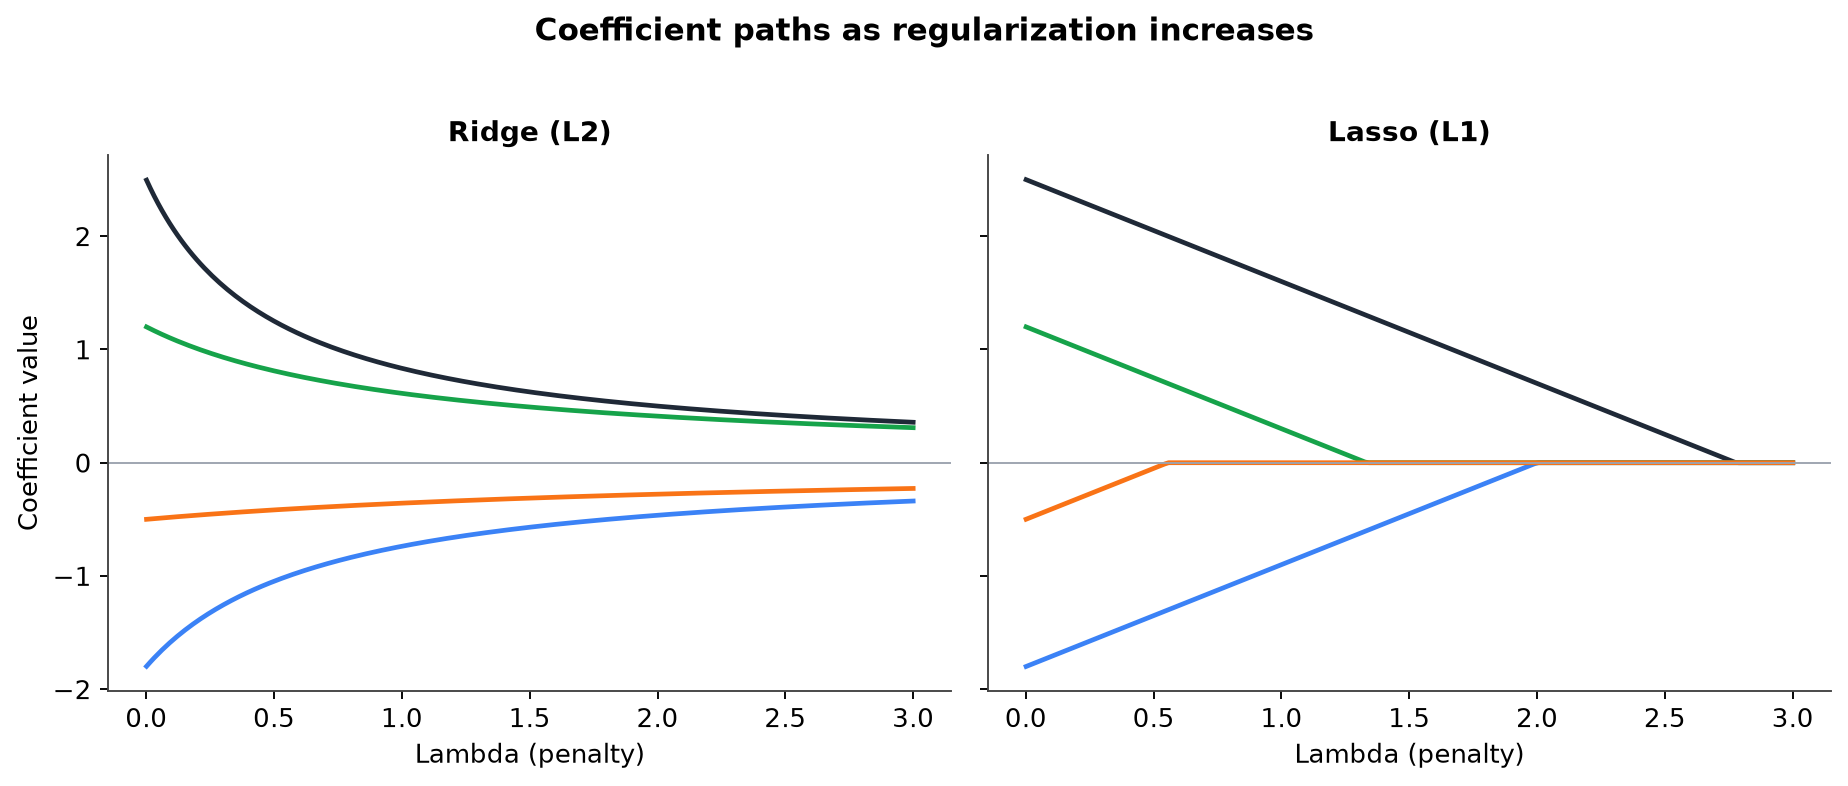
\includegraphics[width=0.55\textwidth]{../book/_static/generated/figures/en/regularization_paths.png}
  \end{center}
\end{frame}

\begin{frame}{Ridge on real data: the \textit{Credit} dataset}
  \begin{itemize}
    \item As $\lambda$ increases, coefficients shrink toward zero
    \item Trades a small increase in bias for a reduction in variance
  \end{itemize}
  \begin{center}
    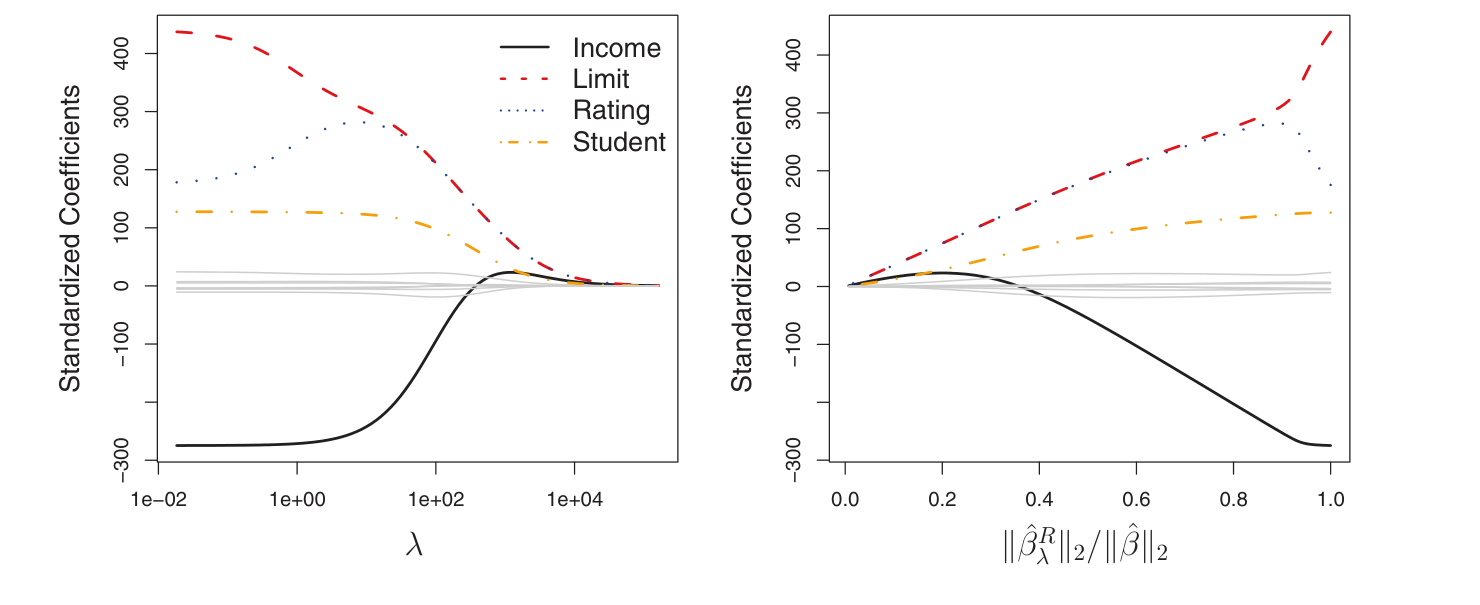
\includegraphics[width=0.6\textwidth]{../book/_static/book_figures/islr_fig6_4_ridge_credit.png}
  \end{center}
  \fuente{James, Witten, Hastie \& Tibshirani (2013), \textit{An Introduction to Statistical Learning}, Fig. 6.4.}
\end{frame}

\begin{frame}{Validation and diagnostics in regression}
  \begin{itemize}
    \item \textbf{MSE / RMSE}: mean squared error (and its root); heavily penalizes large errors
    \item \textbf{MAE}: mean absolute error; more robust to outliers
    \item \textbf{$R^2$}: proportion of variance explained by the model (1 = perfect, 0 = as good as predicting the mean)
    \item \textbf{Validation curves}: plotting training and validation error against complexity reveals high bias (both errors high) or high variance (a gap between them)
  \end{itemize}
\end{frame}

\begin{frame}{Summary: 2.1 Regression}
  \begin{itemize}
    \item \textbf{Linear regression}: simple yet very powerful
    \item \textbf{OLS}: exact solution; \textbf{gradient descent}: general and scalable
    \item \textbf{Polynomial regression}: captures non-linear relationships, at the cost of more overfitting risk
    \item \textbf{Regularization}: Ridge shrinks, Lasso selects variables
  \end{itemize}
\end{frame}

% ============================================================
\section{2.2 Classification}

\begin{frame}{Classification: predicting categories}
  \begin{itemize}
    \item The goal is to predict a \textbf{category}, not a continuous number
    \item Examples: spam vs. not-spam, sick vs. healthy, cat vs. dog vs. bird
    \item \textbf{Logistic regression} starts by estimating the \textbf{probability} of belonging to a class
  \end{itemize}
\end{frame}

\begin{frame}{The sigmoid function}
  \begin{itemize}
    \item Maps any real value to a probability between 0 and 1
    \item $\sigma(t) = \dfrac{1}{1+e^{-t}}$, where $t$ is the \textit{logit} (a linear combination of the features)
    \item Trained by minimizing \textbf{cross-entropy} (log loss) with gradient descent
  \end{itemize}
  \begin{center}
    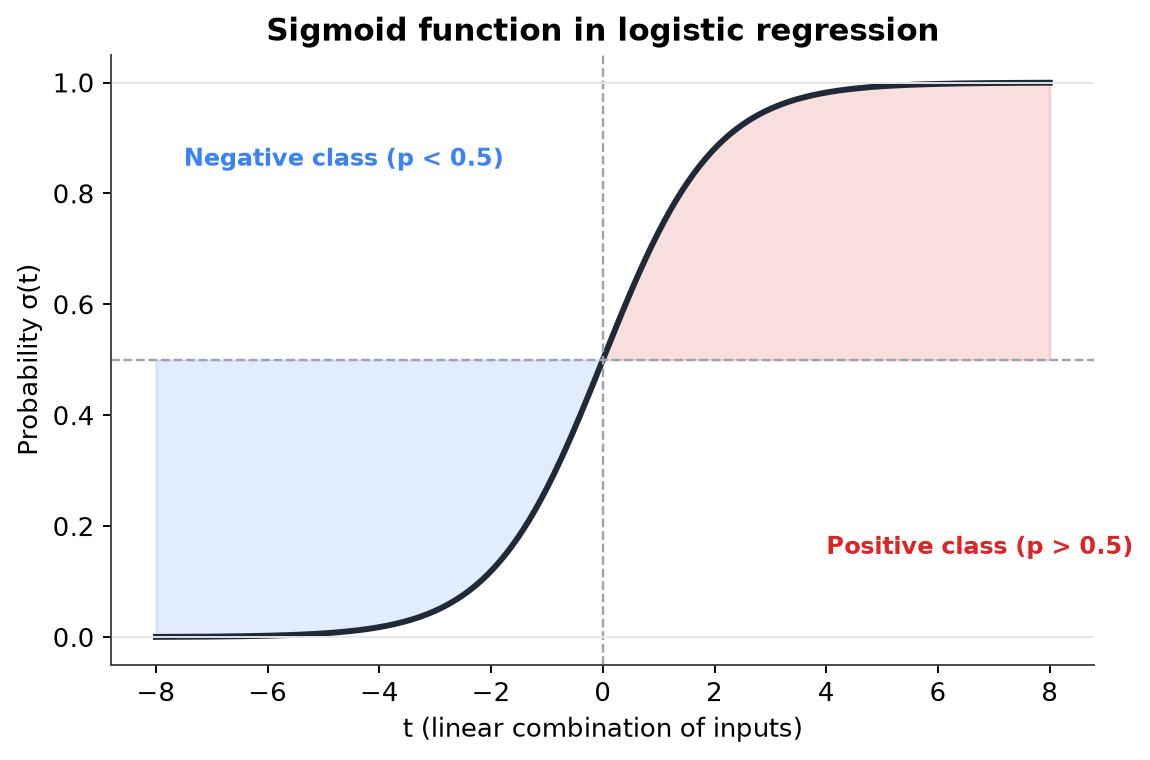
\includegraphics[width=0.42\textwidth]{../book/_static/generated/figures/en/sigmoid_function.png}
  \end{center}
\end{frame}

\begin{frame}{Why not use linear regression?}
  \begin{itemize}
    \item Linear regression can predict probabilities $<0$ or $>1$ (nonsensical)
    \item Logistic regression uses the sigmoid to keep the output always within $[0,1]$
  \end{itemize}
  \begin{center}
    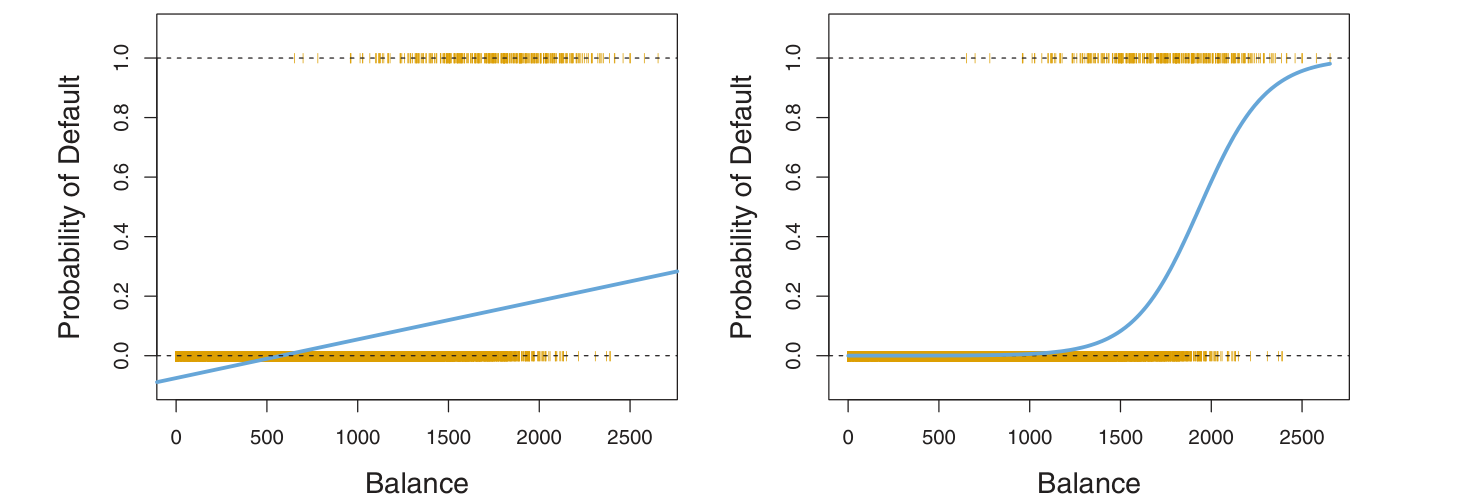
\includegraphics[width=0.62\textwidth]{../book/_static/book_figures/islr_fig4_2_default_logistic.png}
  \end{center}
  \fuente{James, Witten, Hastie \& Tibshirani (2013), \textit{An Introduction to Statistical Learning}, Fig. 4.2.}
\end{frame}

\begin{frame}{Decision trees}
  \begin{columns}
    \begin{column}{0.45\textwidth}
      \begin{itemize}
        \item Split the feature space with successive orthogonal cuts, like a flowchart of yes/no questions
        \item \textbf{CART} algorithm: each split maximizes the purity of the child nodes (Gini index or entropy)
        \item Easy to interpret, but prone to overfitting without \textbf{pruning}
      \end{itemize}
    \end{column}
    \begin{column}{0.5\textwidth}
      \centering
      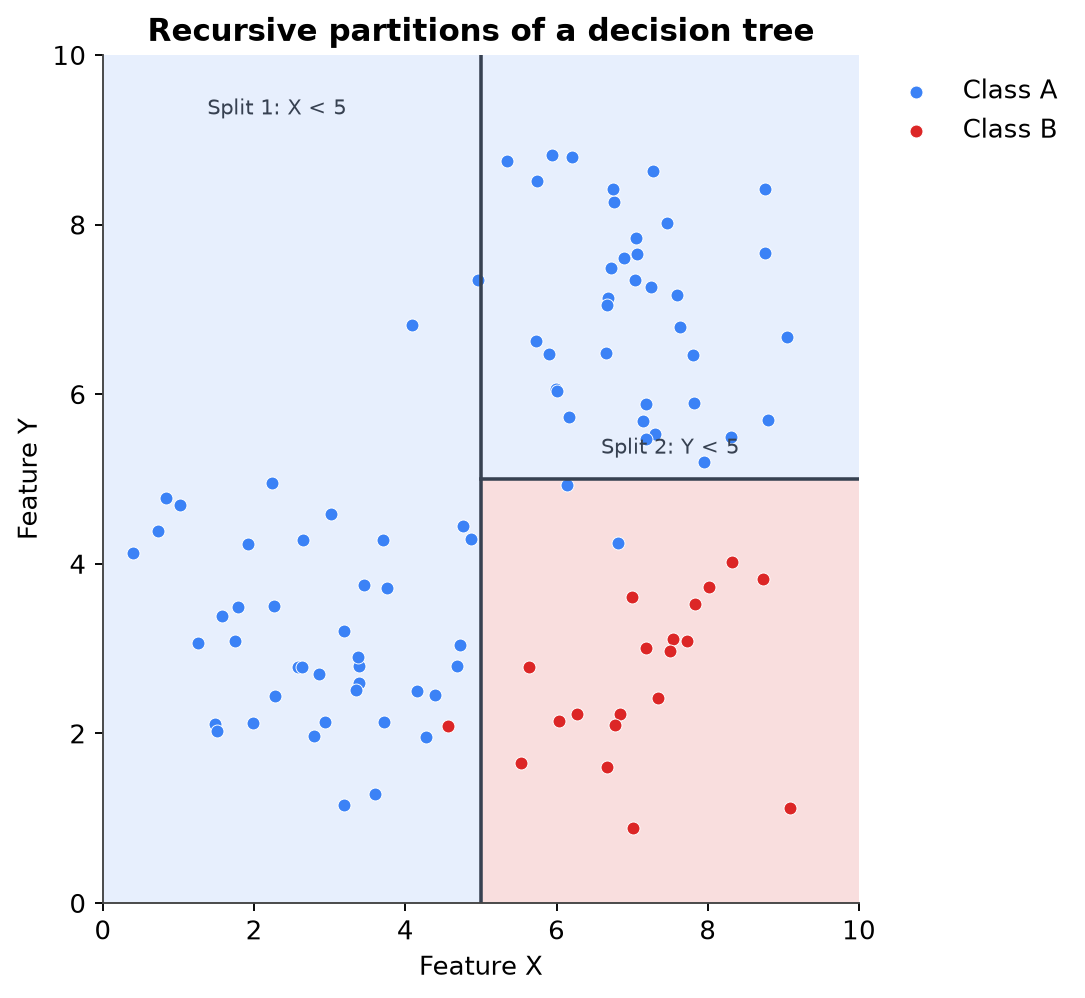
\includegraphics[width=\textwidth]{../book/_static/generated/figures/en/decision_tree_partition.png}
    \end{column}
  \end{columns}
  \ejemplo{``does the email contain the word `free'? $\rightarrow$ yes $\rightarrow$ does it have more than 3 links? $\rightarrow$ yes $\rightarrow$ spam.''}
\end{frame}

\begin{frame}{Random Forests}
  \begin{itemize}
    \item Combine \textbf{many trees} to reduce variance and improve robustness
    \item \textbf{Bagging}: each tree is trained on a different \textit{bootstrap} sample (with replacement)
    \item \textbf{Decorrelation}: only a random subset of features is considered at each split
  \end{itemize}
  \footnotesize
  Several bootstrap samples, a different tree per sample, and predictions combined by majority vote or averaging.
  \begin{center}
    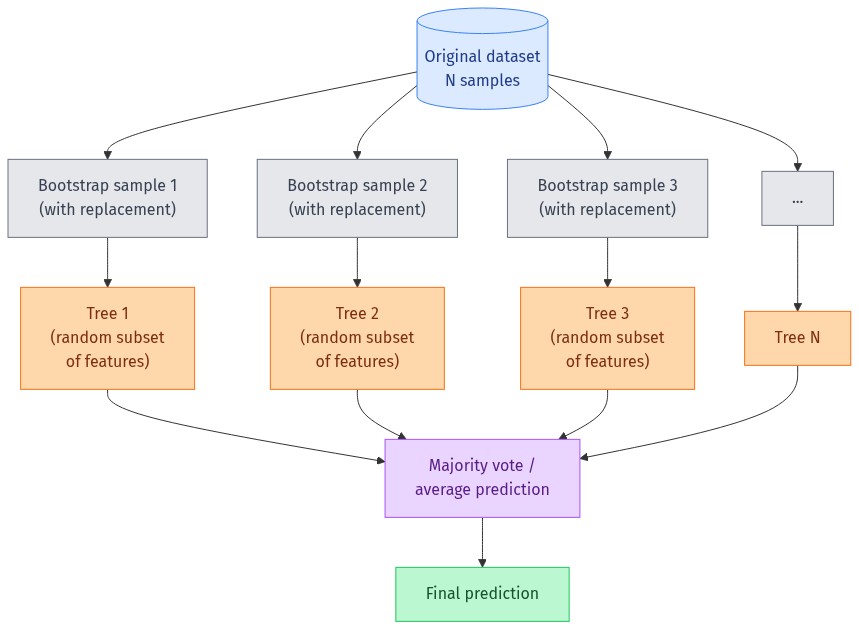
\includegraphics[width=0.5\textwidth]{../book/_static/generated/diagrams_pdf/en/01_supervised_learning_02_classification_01.png}
  \end{center}
\end{frame}

\begin{frame}{SVM: maximum margin}
  \begin{columns}
    \begin{column}{0.45\textwidth}
      \begin{itemize}
        \item Finds the \textbf{hyperplane} that separates the classes with the \textbf{maximum margin}
        \item \textbf{Support vectors} are the only points that determine the boundary
        \item The \textit{kernel trick} enables non-linear boundaries, mapping the data into a higher-dimensional space
      \end{itemize}
    \end{column}
    \begin{column}{0.5\textwidth}
      \centering
      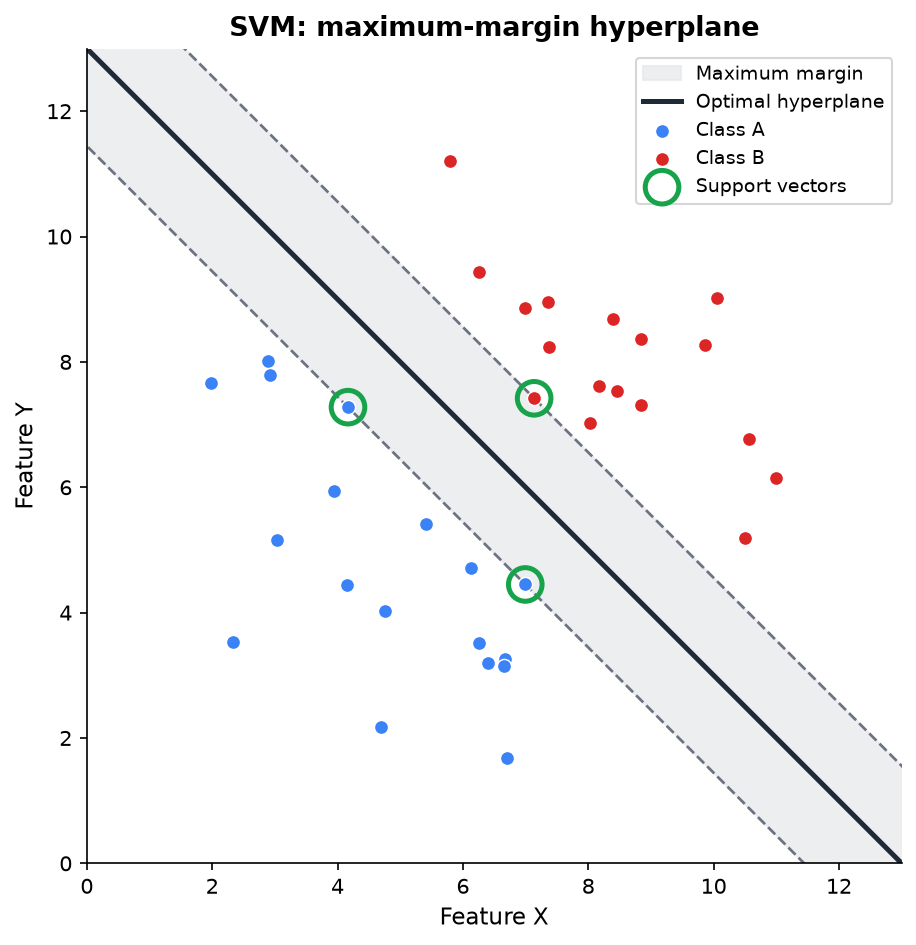
\includegraphics[width=\textwidth]{../book/_static/generated/figures/en/svm_margin.png}
    \end{column}
  \end{columns}
\end{frame}

\begin{frame}{Voting and stacking}
  \begin{itemize}
    \item Combine \textbf{several models} to get a better prediction than any single one
    \item \textbf{Voting}: majority vote or average of probabilities, with a fixed rule
    \item \textbf{Stacking}: a meta-model \textbf{learns} how to combine the base models' outputs
  \end{itemize}
  \begin{center}
    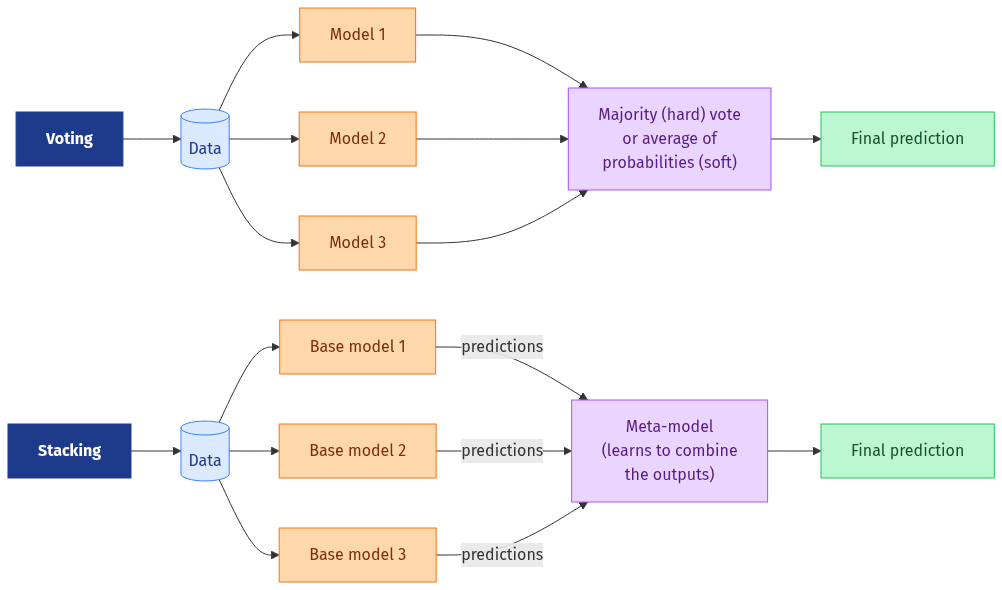
\includegraphics[width=0.68\textwidth]{../book/_static/generated/diagrams_pdf/en/01_supervised_learning_02_classification_03.png}
  \end{center}
\end{frame}

\begin{frame}{Boosting}
  \begin{itemize}
    \item Unlike the parallel training of random forests, boosting trains models \textbf{sequentially}
    \item Each new model tries to correct the previous one's errors, weighting misclassified instances more heavily
    \item Modern examples: XGBoost, Gradient Boosting
  \end{itemize}
  \begin{center}
    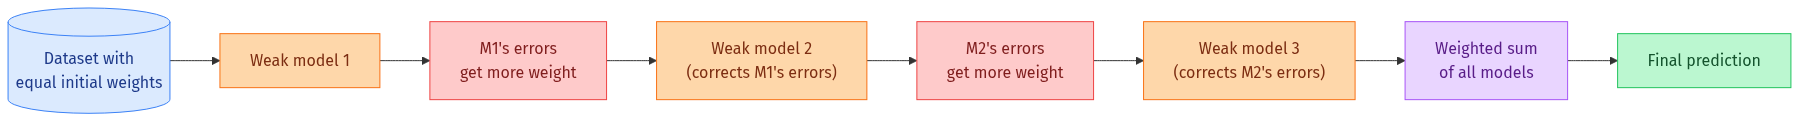
\includegraphics[width=0.85\textwidth]{../book/_static/generated/diagrams_pdf/en/01_supervised_learning_02_classification_02.png}
  \end{center}
\end{frame}

\begin{frame}{Neural networks}
  \begin{itemize}
    \item Layers of neurons connected by adjustable weights
    \item Each neuron applies a non-linear activation function: \textbf{ReLU} in hidden layers, \textbf{Softmax} in the output layer
    \item \textbf{Backpropagation}: propagates the error backward from the output to adjust every weight
  \end{itemize}
  \begin{center}
    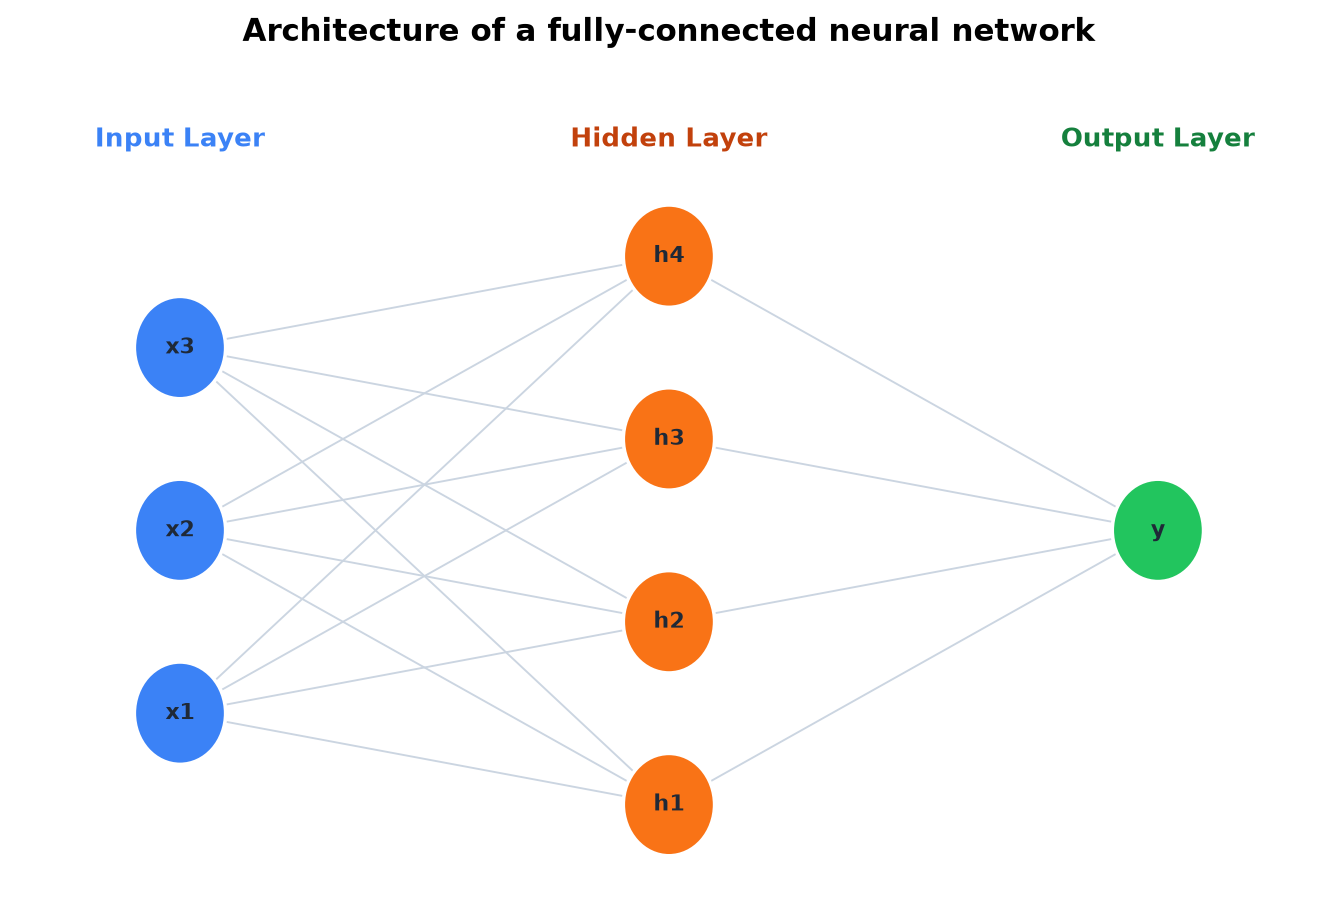
\includegraphics[width=0.42\textwidth]{../book/_static/generated/figures/en/nn_architecture.png}
  \end{center}
\end{frame}

\begin{frame}{Evaluating classifiers}
  \begin{itemize}
    \item \textbf{Accuracy}: can be misleading when classes are imbalanced
    \item \textbf{Precision} and \textbf{recall}: how reliable are the positives vs. how many real positives are found
    \item \textbf{F1}: a balance between both
    \item \textbf{ROC-AUC}: compares models without depending on a fixed threshold
  \end{itemize}
  \ejemplo{\footnotesize if 99\% of transactions aren't fraud, a model that always says ``not fraud'' would have 99\% accuracy without having learned anything useful.}
  \begin{center}
    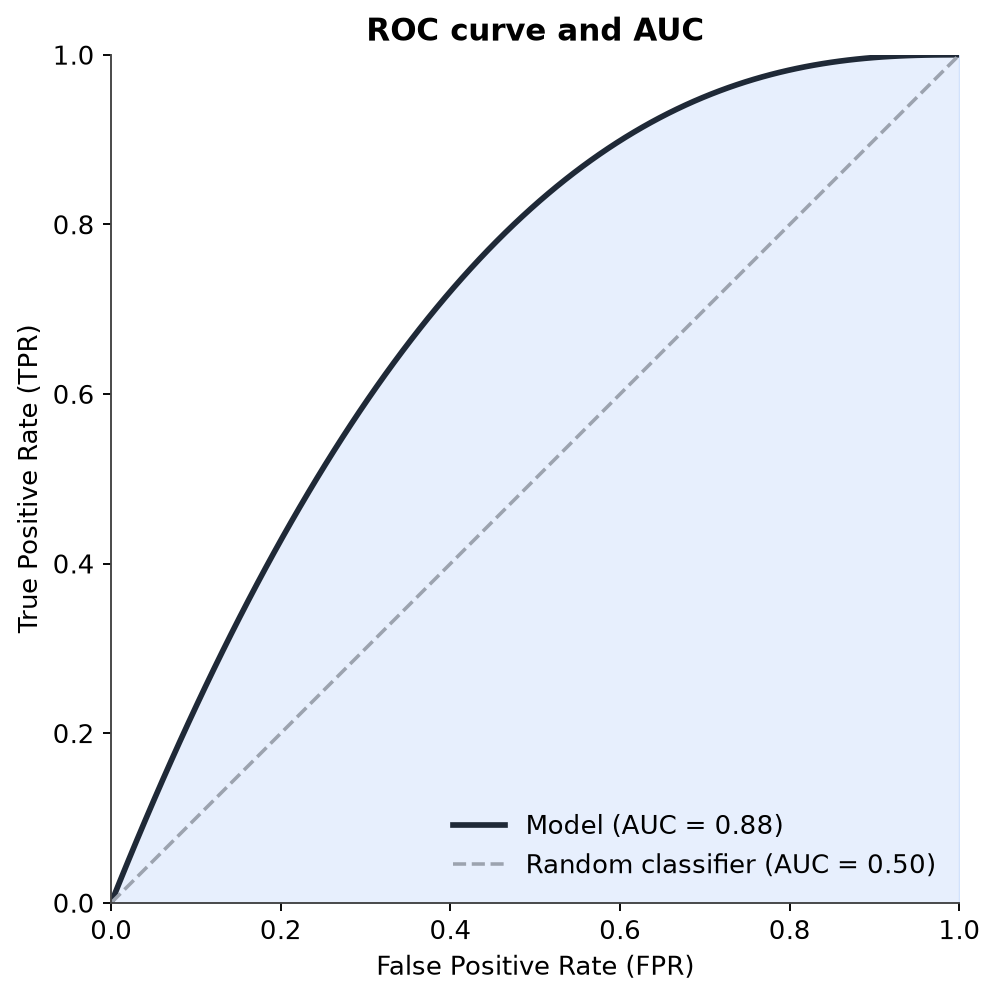
\includegraphics[width=0.26\textwidth]{../book/_static/generated/figures/en/roc_curve.png}
  \end{center}
\end{frame}

\begin{frame}{Training and diagnostic strategies}
  \begin{itemize}
    \item \textbf{Beat a baseline}: before going complex, check you beat a trivial (random) classifier
    \item \textbf{Learning curves}: training/validation loss and accuracy reveal the exact point of overfitting
    \item \textbf{Early stopping}: stop training once validation stops improving
    \item \textbf{Error analysis}: manually inspect the cases where the model fails
  \end{itemize}
\end{frame}

\begin{frame}{Summary: 2.2 Classification}
  \begin{itemize}
    \item \textbf{Logistic regression}: extends linear regression to probabilities
    \item \textbf{Trees}: interpretable, prone to overfitting; \textbf{Random Forest} fixes it by combining many
    \item \textbf{SVM}: optimal separation, with the kernel trick for complex boundaries
    \item \textbf{Ensembles} (voting, stacking, boosting): combine models to improve performance
    \item \textbf{Neural networks}: powerful but harder to interpret
  \end{itemize}
\end{frame}

\begin{frame}
  \centering
  {\Huge End of Chapter 2}\\[1em]
  {\large Next: Chapter 3 --- Unsupervised Learning}
\end{frame}

\end{document}
